\chapter{Methodology}
\label{c:method}

HiHi Iam r44~. The organization of this thesis is as follows. In chapte~\ref{c:thm}, the theoretical background and definition of surface plasmon will be included~\cite{LeeWave}. Chapte~\ref{c:exp} contains description of experiment methods such as atomic force microscopy and scanning electron microscopy. 

%==========================================================================================
\section{Problem Setup}
\label{s:probsetup}
There are a query set $Q={\{q_1,q_2,...,q_T\}}\subset\mathbb{R}^D$ at the server $P$ and a dataset $X_i\subset\mathbb{R}^D$ on each local machine $M_i$.  For each coming query $q_t$, we want to find its $k_{th}$ nearest neighborhood among these distributed datasets while reducing the transmission cost between $P$ and each $M_i$.

%==========================================================================================
\section{Overview of Our Framework}
\label{s:overview}
In this section, we describe the overall framework of our work.  Then, we will give the details about the framework in the following sections.

\begin{figure}[htpb!]
  \centering
    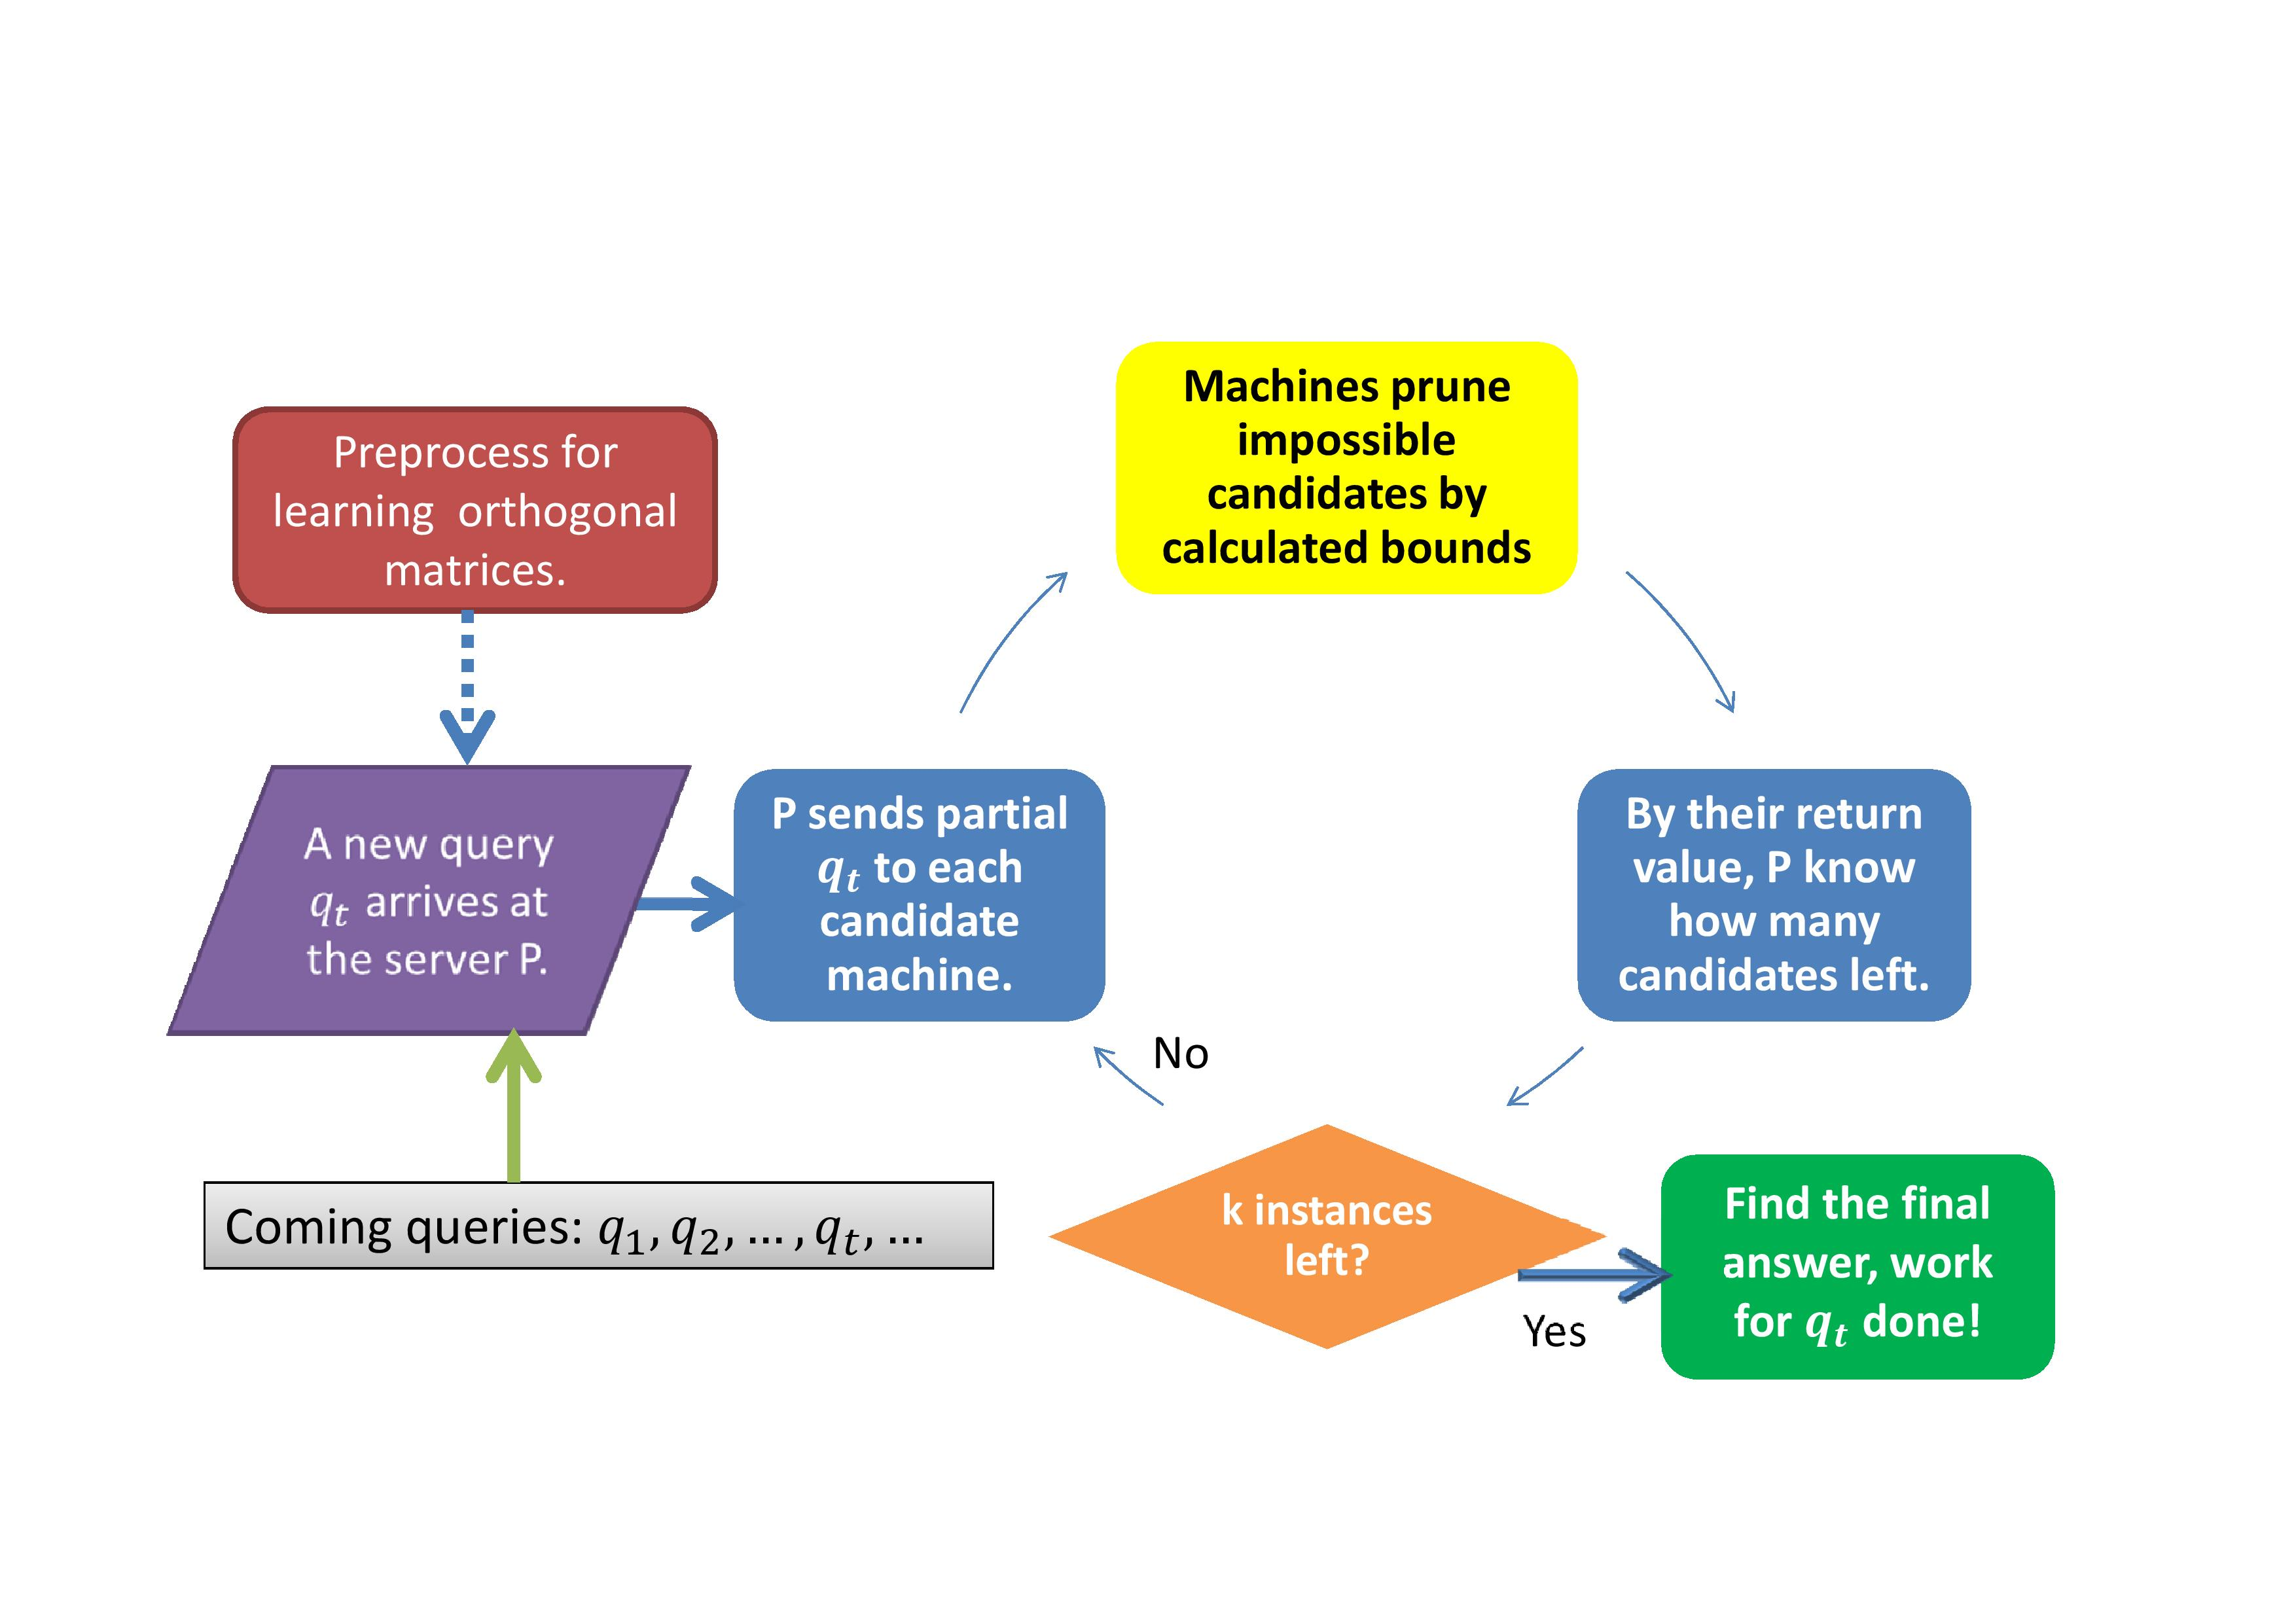
\includegraphics[width=1.0\textwidth]{fig/flow.jpg}
    \caption{\label{fig:flow}The overall flow of our framework.}
\end{figure}

Figure~\ref{fig:flow} is the overall flow on our framework.  There are two main phases in our framework.  For each $X_i$, the first phase only needs to be done for once.  On the other hand, we need to run the second phase for each new query $q_t$.

The first phase is an preprocessing procedure for the second phase. Its goal is to improve the performance of pruning in the second phase.  We will prove in the section \ref{ss:derivation_of_the_bounds} that this pruning power is highly correlated to the distribution of the norm of the feature vectors. As a result, each $M_i$ would learn an othorogal matrix $W_i$ for its $X_i$ to fit our desired distribution and then send each $W_i$ back to $P$.  We can notice that this phase is only dependent on $X_i$ and independent of $q_t$.  Therefore, we only need to do the first phase for once.  we give the details about how to learn $W_i$, how to send it back to $P$ in the section \ref{s:orthogonal}.

The second phase is the main procedure of our framework.  Note that $P$ have already got $W_i$ for each $X_i$ in the beginning of the second phase. For each coming query $q_t$, we iteratively prune some candidates which are impossible to be the $k$NN of $q_t$ to reduce the search space until there are only $k$ candidates left.

To prune candidates iteratively, we divide the second phase into several rounds.  For each round $j$, we use a $Select$ function $S_i(q_t,j;\theta_t)$ to generate the values for trasmitting from $P$ to $M_i$, where $S_i$ is the importance-selecting function of $M_i$ and $\theta_t$ is its parameters for $q_t$.  (We put the details of $S_i$ at the section \ref{s:importance_selecting_function}.)  By these values, each $M_i$ could calculate the bounds between each candidate $x_l$ and $q_t$.  With these bounds, $P$ would be able to determine which candidates are definitely not our answer and then disregards them in the following rounds.  By these pruning, we could achieve the goal of saving transmission cost from avoiding to consider the unnecessary candidates.

Note that we could use the square of the Euclidean distance instead of the origin Euclidean distance to find $k$NN as it is non-negative.  So we will use the former one in our framework.

%==========================================================================================
\section{Orthogonal Transformation}
\label{s:orthogonal}
Since the In this section, we describe the overview of this thesis.

%==========================================================================================
\subsection{Definition of Ortohogonal Transformation}
\label{ss:ortho_def}
\newtheorem{Orthogonal}{\bf Definition}
\begin{Orthogonal}
A matrix $W \in\mathbb{R}^{D\times D}$ is orthogonal if whose columns and rows are orthogonal vectors, i.e.
\[
W^{T}W=WW^{T}=I
\]
where $I$ is the identity matrix.
\end{Orthogonal}

%==========================================================================================
\subsection{Property of Orthogonal Transformation}
\label{ss:ortho_prop}
\newtheorem{ProOfOrthogonal}{\bf Property}
\begin{ProOfOrthogonal}
Let $x, y\in\mathbb{R}^{D\times 1}$, and $W\in\mathbb{R}^{D\times D}$ be an orthogonal matrix. Then,
\[
Dist(x,y)=\sum^D_{d=1}{(x[d]-y[d])^2} \\
=\sum^D_{d=1}{(W[d,:]x-W[d,:]y)^2}=Dist(Wx,Wy)
\]
where $W[d,:]$ is the $d_{th}$ row of $W$.
\end{ProOfOrthogonal}

We will use this important property in the section \ref{sub:reduce_the_norm_with_orthogonal_transformation}.

%==========================================================================================
\section{Enhance the Bounds by the Orthogonal Transformation}
\label{s:ortho_bounds}
In the section \ref{s:overview}, we mentioned that the first phase is an auxiliary step for the second phase.  After the introduction of the orthogonal transformation, we introduce this powerful tool into the first phase in our framework.

\subsection{The Goal of the First Phase} % (fold)
\label{ss:the_goal_of_the_first_phase}

Our goal in the first phase is to reduce the ranges of the bounds used in the second phase.  Since we will use a threshold to prune the impossible candidates according to their bounds in the pruning procedure, the ranges of the bounds would be one of the most influential factor of the pruning power. It is easy to understand that when the ranges of their bounds is short, more candidates would be pruned than those with long ranges of the bounds.  In other words, the shorter the range of the bound, the higher chance this candidate would be pruned if it is not our final answer of $k$NN.  

Moreover, we would prove in the section~\ref{ss:reduce_the_norm_with_orthogonal_transformation} that to reduce the range of the bounds, the final goal of the first phase would become to learn an orthogonal transformation $W$ which could make each raw feature vector $x\in \mathbb{R}^D$ (the orange vector in the figure below) transformed to be $Wx$ (the red vector in the figure below) which would make the absolute values of elements in the forward part of the vector larger and those in the later part smaller.
\begin{figure}[htpb!]
  \centering
    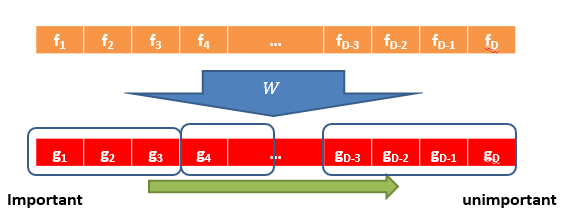
\includegraphics[width=0.8\textwidth]{fig/important.png}
    \caption{\label{fig:flow}The goal of the first phase.}
\end{figure}


% subsection the_goal_of_the_first_phase (end)

\subsection{Definition of the Bounds} % (fold)
\label{ss:definition_of_the_bounds}

First, we need to define the bounds for the pruning.  Recall that given a query $q_t$, our goal is to find its $k$NN in these distributed datasets $X_i$.  Intuitively, we need to calculate the square of the Euclidean distance $Dist(q_t,x), \forall x\in \cup_i X_i$.  However, to cacluate $Dist(q_t,x)$, we need to send the whole $q_t$ to the local machines or send the whole $x$ to $P$, which causes a huge transmission cost.  Therefore, instead of the exact value of Euclidean distances, our propsed framework uses bounds to find the $k$NN.

\newtheorem{Bounds}{\bf Definition}
\begin{Bounds}
$\forall x,y \in \mathbb{R}^D$, a lower bound $LB(x,y)$ and a upper bound $UB(x,y)$ must satisfy the following inequation:
\[
LB(x,y)\leq Dist(x,y) \leq UB(x,y)
\]
\end{Bounds}

\subsection{Relation Between the Norms and the Bounds} % (fold)
\label{sub:relation_between_the_norms_and_the_bounds}

To acheive the goal of reducing the length of the ranges of the bounds, we could look into the derivation of the bounds. Suppose there are two vectors $x,y\in \mathbb{R}^D$, but we could only observe the first $s$ dimensions of $x$ and $\sum^D_{d=s+1}{x[d]^2}$, which is the square of two norm of the unobserved part $x[s+1:D]$.  In the section \ref{ss:derivation_of_the_bounds}, we give the bounds as 
{
\begin{eqnarray*}
\lefteqn{LB(x,y) = \sum^s_{d=1}{(x[d]-y[d])^2}.} \label{eq:single-LB-tmp} \\
\lefteqn{UB(x,y) = \sum^s_{d=1}{(x[d]-y[d])^2}} \notag \\
& + & \sum^D_{d=s+1}{x[d]^2}+\sum^D_{d=s+1}{y[d]^2} \notag \\
& + & 2 \times \sqrt{\sum^D_{d=s+1}{x[d]^2}\times \sum^D_{d=s+1}{y[d]^2}.}\label{eq:single-UB-tmp}
\end{eqnarray*}
}

Therefore, we could get the length of the range by the substraction.
{
\begin{eqnarray*}
\lefteqn{Len = UB(x,y) - LB(x,y)}\\
& = \sum^D_{d=s+1}{x[d]^2}+\sum^D_{d=s+1}{y[d]^2} \\
& + 2 \times \sqrt{\sum^D_{d=s+1}{x[d]^2}\times \sum^D_{d=s+1}{y[d]^2}.}\label{eq:len-range}
\end{eqnarray*}
}
Since the term $\sum^D_{d=s+1}{x[d]^2}$ is given, all we could do is to reduce the length with the help of the $\sum^D_{d=s+1}{y[d]^2}$ term.  If we could reduce $\sum^D_{d=s+1}{y[d]^2}$, the term $\sum^D_{d=s+1}{x[d]^2}\times \sum^D_{d=s+1}{y[d]^2}$ would also decrease and then make $Len$ smaller.  Therefore, our goal now becomes to make the term $\sum^D_{d=s+1}{y[d]^2}$ as small as possible, which is the square norm of the vector $y[s+1:D]$.

Note that the lower (upper) bounds is non-decreasing (non-increasing) as $s$ becomes larger and $LB(x,y)=UB(x,y)$ when $s=D$.  This means that $LB$ and $UB$ would be exactly equal to $\sum^D_{d=1}{(x[d]-y[d])^2}$ eventually.

To reduce the length of the ranges $Len$ for each $s$, we hope to make $\sum^D_{d=s+1}{y[d]^2}$ as small as possible.  However, since the feature vector $y$ is given from datasets, the value of $\sum^D_{d=s+1}{y[d]^2}$ is already  determined when $s$ is given.  As a result, we introduce the orthogonal transformation to achieve this goal.

% subsection relation_between_the_norms_and_the_bounds (end)


\subsection{Equivalent Bounds After Transformation} % (fold)
\label{sub:equivalent_bounds_after_transformation}

From the section \ref{ss:ortho_prop}, we know the distance of two vectors won't be changed after an orthogonal transformation.  Now we use this property to achieve our goal to reduce the length of the ranges $Len$ given $s$.

Given an orthogonal transformation $W\in\mathbb{R}^{D\times D}$, we have $Dist(x,y)=Dist(Wx,Wy)$.  This means that the bounds we derivated before could also be the bounds for $Dist(Wx,Wy)$.  That is,
\[
LB(x,y)\leq Dist(x,y)=Dist(\hat{x},\hat{y}) \leq UB(x,y)
\]
where $\hat{x}=Wx$.

This also means that we could use the same way to derivate the lower bounds and upper bounds for $Dist(Wx,Wy)$ and these bounds are also the bounds for $Dist(x,y)$.  That is,
\[
LB(\hat{x},\hat{y})\leq Dist(x,y)=Dist(\hat{x},\hat{y}) \leq UB(\hat{x},\hat{y})
\]

So, we could use the bounds $LB(\hat{x},\hat{y}),UB(\hat{x},\hat{y})$ for $Dist(x,y)$ and the length of range we want to reduce becomes
{
\begin{eqnarray*}
\lefteqn{\hat{Len}(W) = UB(\hat{x},\hat{y}) - LB(\hat{x},\hat{y})} \\
& = \sum^D_{d=s+1}{\hat{x}[d]^2}+\sum^D_{d=s+1}{\hat{y}[d]^2} \notag \\
& +  2 \times \sqrt{\sum^D_{d=s+1}{\hat{x}[d]^2}\times \sum^D_{d=s+1}{\hat{y}[d]^2}.}\label{eq:len-range-hat}
\end{eqnarray*}
}
which becomes a function of $W$.

As a result, instead of trying to reduce $\sum^D_{d=s+1}{y[d]^2}$ which is impossible as we mentioned in the section \ref{sub:relation_between_the_norms_and_the_bounds}, our goal becomes to reduce $\sum^D_{d=s+1}{\hat{y}[d]^2}$ with the help of $W$.

% subsection equivalent_bounds_after_transformation (end)

\subsection{Reduce the Norm with Orthogonal Transformation} % (fold)
\label{ss:reduce_the_norm_with_orthogonal_transformation}

For $y\in \mathbb{R}^{D\times 1}$ and $W\in\mathbb{R}^{D\times D}$, given $s$, we want to reduce $\sum^D_{d=s+1}{\hat{y}[d]^2}$ as much as possible.  However, since $s$ is unknown while deciding $W$ in the first phase of our framework, we have to handle all possible values which $s$ could be.  Moreover, since $\sum^D_{d=1}{\hat{y}[d]^2}$ is equal to $\sum^D_{d=1}{y[d]^2}$, which is independent with $W$, if the $\sum^D_{d=s+1}{\hat{y}[d]^2}$ decreases with some $W$, the term $\sum^s_{d=1}{\hat{y}[d]^2}$ must increase.  Here, we use a more general strategy to deal with these problems.

We could look the term $\sum^D_{d=s+1}{\hat{y}[d]^2}$ from a different angle.  Actually, this term is the square norm of the latter part of the vector $\hat{y}$. Therefore, although $\sum^D_{d=1}{\hat{y}[d]^2}$ is a constant for $W$, we could reduce the square norm of the latter part by increasing the forward part of it.  In other words, we move the norm of the latter part of $y$ to its forward part.  To accomplish it, we design an objective function and then optimize this function to find our ideal $W$.

\begin{equation}\label{objective}
	f(W;y)=\sum^D_{d=1}{w_d\times\hat{y}[d]^2}=\sum^D_{d=1}{w_d\times(W[d,:]y[d])^2}
\end{equation}
where $w_d=d,  \forall d=1:D$.

Because $w_d$ would give the larger penalty as $d$ increases, the elements in the latter part of $\hat{y}$ would be forced to become small while minimizing this objective function.  This is exactly our goal to reduce $\sum^D_{d=s+1}{\hat{y}[d]^2}$.  Therefore, our question becomes how to optimize this objective function with the constraints that $W$ must be an orthogonal matrix.


% subsection reduce_the_norm_with_orthogonal_transformation (end)

\subsection{Optimize with Orthogonal Constraints} % (fold)
\label{ss:optimize_with_orthogonal_constraints}

Finally, we could introduce this concept of reducing the norms into our framework.  In the first phase, we solve the following optimization problem to learn an orthogonal matrix $W_i$ for each machine $Mi$.

\begin{equation}
\begin{aligned}
& \underset{W}{\text{minimize}}
& & F_i(W) \\
& \text{subject to}
& & W^{T}W=WW^{T}=I
%& & W \leq b_i, \; i = 1, \ldots, m.
\end{aligned}
\end{equation}

where 
\begin{equation}\label{objective-F}
	F_i(W)=\sum_{x \in X_i}{f(W;x)}\\
	=\sum_{x \in X_i}{ \sum^D_{d=1} {d\times(W[d,:]x[d])^2} }
\end{equation}.

This is an optimization problem with constraints that its solution must be an orthogonal matrix.  We could solve it efficiently with the help of the package from~\cite{Fopt} as long as we have its gradient. 

After we get the optimal $W^*_i$ for each $M_i$, we send these matrices back to the server $P$.  Since the learning of $W^*_i$ is independent with the queries in the future, we only have to go through the procedure of learning $W^*_i$ for once if $X_i$ doesn't change too much.

% subsection optimize_with_orthogonal_constraints (end)

\subsection{Reduce the Cost of Sending Matrices} % (fold)
\label{ss:reduce_the_cost_of_sending_matrices}
%http://math.stackexchange.com/questions/375344/parameters-to-represent-degrees-of-freedom-in-n-times-n-orthogonal-real-matric
%http://math.stackexchange.com/questions/28189/freedoms-of-real-orthogonal-matrices

However, the cost to sending an orthogonal matrix $W\in\mathbb{R}^{D\times D}$ is $D\times D$, which is too expensive.  Therefore, in this section, we prove that we could reduce this cost to $\frac{D\times (D-1)}{2}$.

First, we introduce a lemma which would be used in our proof.

\newtheorem*{lemma}{Lemma}
\begin{lemma}\normalfont
 For all vector $\bold{x}=(x_1,x_2,\ldots,x_D)\in\mathbb{R}^D$, we could use a spherical coordinate system with a radial coordinate $r$ and $D-1$ angular coordinates $\phi_1, \phi_2, ..., \phi_{D-1}$ to represent it as
\begin{itemize}
	\item $x_1 = r cos(\phi_1)$
	\item $x_2 = r sin(\phi_1)cos(\phi_2)$
	\item $x_3 = r sin(\phi_1)sin(\phi_2)cos(\phi_3)$
	\item ~\vdots
	\item $x_{D-1} = r sin(\phi_1)\ldots sin(\phi_{D-2})cos(\phi_{D-1})$
	\item $x_{D} = r sin(\phi_1)\ldots sin(\phi_{D-2})sin(\phi_{D-1})$
\end{itemize}
where $\phi_i\in[0,\pi],~\forall i=1,2,...,D-2$ and $\phi_{D-1}\in[0,2\pi)$. $\blacksquare$
\end{lemma}

Since these row vectors in $W$ are orthonomal vectors, their $r$ in this lemma is $1$, which allows us to represent an orthonomal vector in $\mathbb{R}^D$ with $D-1$ parameters ($\phi_1,\phi_2, ...,\phi_{D-1}$ in the lemma).  Moreover, 

Now we are ready to give the proof by mathematical induction.

\newtheorem*{half}{Theorem}
\begin{half}\normalfont
Given an orthogonal transformation $W\in\mathbb{R}^{D\times D}$, we could use $\frac{D\times (D-1)}{2}$ parameters to construct $W$.
\end{half}

\newtheorem*{mproof}{Proof}
\begin{mproof}\normalfont
Base case $d=2$: If $d=2$, we 
 Given an orthogonal transformation $W\in\mathbb{R}^{D\times D}$, we could use $\frac{D\times (D-1)}{2}$ parameters to construct $W$.
\begin{enumerate}
	\item gaga
	\item ff
\end{enumerate}
\end{mproof}$\blacksquare$

% subsection reduce_the_cost_of_sending_matrices (end)


%==========================================================================================
\section{Prune by the Bounds}
\label{s:prune}
Now we start to discuss the second phase of our framework.  In this section, we talk about how to prune the candidates if we already have bounds.  Note that this mechanism is the most crucial part to achieve our goal to save the transmission cost.

% subsection definition_of_bounds (end)

\subsection{Prune the Candidates with the Bounds} % (fold)
\label{ss:prune_the_candidates_with_the_bounds}

For the query $q_t$, if we already know $LB(q_t,x)$ and $UB(q_t,x)$ $\forall x\in \cup_i X_i$, we could use the $k_{th}$ smallest upper bounds and directly prune those $x$ whose lower bounds are higher than this value $thr$. I.e., we want to prune
\[
\{x |LB(q_t,x)>thr, \forall x \in \cup_i X_i\}
\]
where $thr$ is the $k_{th}$ largest $UB(q_t,x)$ $\forall x\in \cup_i X_i$.  The following figure is an example of how we prune instances.

\begin{figure}[htpb!]
  \centering
    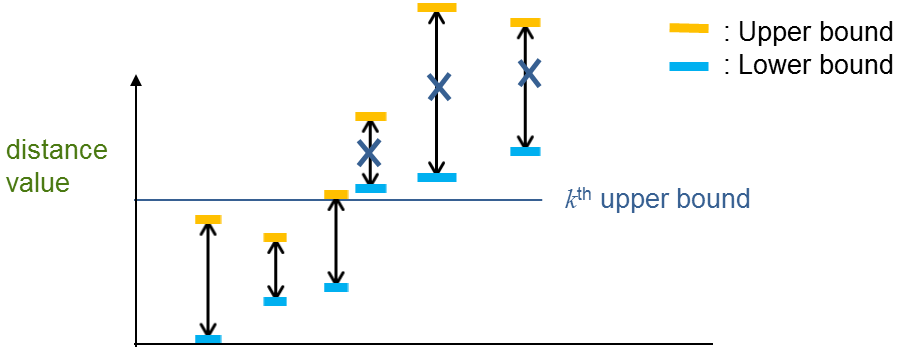
\includegraphics[width=1.0\textwidth]{fig/prune.png}
    \caption{\label{fig:flow}The procedure of pruning impossible candidates.}
\end{figure}

We will talk about the details to generate these bounds and find the threshold in the section \ref{ss:find_the_threshold_in_distributed_machines}.

% subsection prune_the_candidates (end)

\subsection{Derivation of the Bounds} % (fold)
\label{ss:derivation_of_the_bounds}

Suppose there are two vectors $x,y\in \mathbb{R}^D$, we know the square of their Euclidean distance is 
\begin{equation}
	Dist(x,y)=\sum^D_{d=1}{(x[d]-y[d])^2}
\end{equation}

However, if we could only observe the first $s$ dimensions of $x$, we could decompose their distance as 
{
\begin{eqnarray*}
\lefteqn{Dist(x,y)=\sum^D_{d=1}{(x[d]-y[d])^2} } \\
			& &	=\sum^s_{d=1}{(x[d]-y[d])^2} + \sum^D_{d=s+1}{(x[d]-y[d])^2.}	
\end{eqnarray*}
}
Since the first component of \eqref{eq:Eu_decomp} is already known, all we need to do is to deal with the second term. Therefore, we further expand the second term as below:
\[
\sum^D_{d=s+1}{(x[d]-y[d])^2}=\sum^D_{d=s+1}{x[d]^2}+\sum^D_{d=s+1}{y[d]^2}-\sum^D_{d=s+1}{2\times x[d]\times y[d].}
\]

By this analysis, we find the final term is the inner product between two partial vector $x[s+1:D]$ and $y[s+1:D]$, which could be approximated by Cauchy–Schwarz inequality
\begin{equation}\label{eq:Cauchy}
	\sum^D_{d=s+1}{x[d]\times y[d]} \leq \sqrt{\sum^D_{d=s+1}{x[d]^2}\times \sum^D_{d=s+1}{y[d]^2}.}
\end{equation}

After combing with \eqref{eq:Eu_decomp} and \eqref{eq:Cauchy}, we derive the bounds as 
{
\begin{eqnarray}
\lefteqn{LB(x,y) = \sum^s_{d=1}{(x[d]-y[d])^2}.} \label{eq:single-LB} \\
\lefteqn{UB(x,y) = \sum^s_{d=1}{(x[d]-y[d])^2}} \notag \\
& + & \sum^D_{d=s+1}{x[d]^2}+\sum^D_{d=s+1}{y[d]^2} \notag \\
& + & 2 \times \sqrt{\sum^D_{d=s+1}{x[d]^2}\times \sum^D_{d=s+1}{y[d]^2}.}\label{eq:single-UB}
\end{eqnarray}
}
We could notice that the calculation of the bounds only needs the first $s$ dimensions of $x$ and $\sum^D_{d=s+1}{x[d]^2}$.  Therefore, we only need one more number to get the bounds for the unobserved part $x[s+1:D]$.

% subsection derivation_of_bounds (end)

\subsection{Calculation of the Bounds} % (fold)
\label{sub:calculation_the_bounds}
After the derivation of the bounds, we describe the procedure of cacluating them in our framework.  

For the query $q_t$, at the first round (i.e. $j=1$), $P$ sends the first $s_1$ dimensions of $q_t$ and $\sum^D_{d=s_1+1}{q_t[d]}^2$ to each $M_i$ .  With these values, each $M_i$ would able to calculate the lower bounds $LB(q_t,x)$ and upper bounds $UB(q_t,x)$ for each $x\in X_i$.  Then, after $P$ getting the $k_{th}$ smallest upper bounds as $thr$, we could run the pruning procedure.

In each following round (i.e. $j>1$), $P$ sends the next $s_j$ dimensions of $q_t$ to each $M_i$ whose instances were not pruned completely.  These $M_i$ will update their bounds as follows:
{
\begin{eqnarray}
\lefteqn{LB_j(x,y) = LB_{j-1}(x,y)+\sum^{p_j}_{d=p_{j-1}+1}{(x[d]-y[d])^2}.} \label{eq:single-LB} \\
\lefteqn{UB_j(x,y) = LB_{j}(x,y)} \notag \\
& + & \sum^D_{d=p_j+1}{x[d]^2}+\sum^D_{d=p_j+1}{y[d]^2} \notag \\
& + & 2 \times \sqrt{\sum^D_{d=s+1}{x[d]^2}\times \sum^D_{d=s+1}{y[d]^2}.}\label{eq:single-UB}
\end{eqnarray}
}
where $p_j=\sum^j_{i=1}{s_i}$, $LB_j$ and $UB_j$ indicate the lower bounds and upper bounds at the round $j$ repectively.

We call those $p_j$ as pivots, which mean that each machine would observe the first $p_i$ elements of $q_t$ at the round $j$.  

% subsection calculation_the_bounds (end)
\providecommand{\myceil}[1]{\left \lceil #1 \right \rceil }
\providecommand{\myfloor}[1]{\left \lfloor #1 \right \rfloor }

\subsection{Find the Threshold in Distributed Machines} % (fold)
\label{ss:find_the_threshold_in_distributed_machines}
The question now is to find the threshold $thr$ for pruning. In ~\cite{MsWave}, we directly send these bounds computed in each $M_i$ back to the server $P$.  However, it would make the transmission cost grow linearly with the number of total instances in these distributed machines and lead to expensive cost when our dataset is extremely huge.  As a result, we propose a method that could make the growth of the cost independent with the number of total instances.

To be simplified, we could think this problem as follows: given many distribued numbers $N_i$, we want to find the $k_{th}$ largest number among these $N_i$.  The $N_i$ here actually means the upper bounds at the machine $M_i$ in our framework.  Once we model this problem as this, we could solve it through modifying the work of ~\cite{PRP}.

In ~\cite{PRP}, there are also many phases to find the $k$NN.  In the first phase, the server $P$ would send the whole query to every machine.  Then, in the following phases, it just focuses on finding the instances with the $k_{th}$ largest distance with the query.  To make it fit our problem, we can only use the phases of PRP except the first phase to find the $k_{th}$ largest upper bound as our threshold $thr$.  Its cost is linear to
\[
m\times (\myfloor{\frac{k}{|M|}}+1)=m+k,
\] which is much lower than ~\cite{MsWave} when the number of total instances is very large.

%we could estimate the total transmission cost for the single query as following
%\[
%	Cost = \sum^L_{i=1}{T_i\times ResSite_i}+\sum^L_{i=1}{2s_i}
%\]  
%where $T_i$ is the length $q_t$ which was sent , $ResSite_i$ is the number of residual machines, and $s_i$ is the number of residual candidates at the round $i$.


% subsection find_the_threshold_in_distributed_machines (end)
%==========================================================================================

\section{Decide the Pivots} % (fold)
\label{s:decide_the_pivots}

The remaining problem is to decide how many dimensions (i.e. $s_j$) of $q_t$ we have to send from the server $P$ in each round $j$.  If we send too few dimensions, the bounds would be too loose to prune any candidates and we will spend much unnecessary cost in finding the thresholds.  On the other hand, if we send too many dimensions, although it could allow us to prune many candidates at once, it would send too many dimensions to some candidates which could be pruned by much fewer dimensions.  That would also lead to the waste the transmission cost.  Therefore, in this section, we propose a simple but effective method to decide how many dimensions of $q_t$ we should send from $P$ in each round.


\subsection{Estimate the Number of Residual Machines} % (fold)
\label{ss:estimate_the_number_of_residual_machines}

From the discussion above, we could notice that the decision of pivots is highly dependent on the transmission cost.  Therefore, if we could estimate the cost as a cost function of the pivots $p_j$, we could decide these pivots by optimizing this function.

However, to estimate the cost, we need to know the number of residual candidates sites before sending those dimensions of $q_t$ in each round.  But it is almost impossible to know how many sites would be left after we send part of $q_t$ before we actually send the part of $q_t$.  Therefore, we estimate a vector called $EstResMach \in\mathbb{R}^D$ where $EstResMach[j]$ indicates our estimate of the number of residual machines \emph{after} we send $q_t[1:j]$ to each local machine.  

To allow $P$ to  estimate this vector $EstResMach$ without causing any more transmission cost, we use the history information from $q_1,...,q_t$.  Suppose that we just finish finding the answer for $q_t$, during the procedure, we would collect some such pairs of information $(index_j, ResMach_j)$ for some $j$ where $index_j$ means each candidate machine would observe the first $index_j$ dimensions of $q_t$ at the round $j$ and $ResMach_j$ indicates the number of residual machines after pruning by $q_t[1:index_j]$.  For those dimensions which are not in these pairs, we use linear interpolation to estimate their $ResMach$.  

Here(fig?) is an example for the above procedure.



We use the following procedure to maintain this vector $EstResMach$:





% subsection estimate_the_number_of_residual_machines (end)



\subsection{Estimate the Transmission Cost} % (fold)
\label{ss:estimate_the_transmission_cost}

Once we have the vector $EstResMach$, we are ready to estimate the transmission cost \emph{before} sending the query.  For a query $q$, we could estimate its transmission cost in the first round 
\[
Cost_1 = TotalNumOfMach\times s_1 + Cost_{PRP}(TotalNumOfMach)
\]
And for those round $j>1$ as follows,
\[
Cost_j = EstResMach[p_{j-1}]\times s_j + Cost_{PRP}(EstResMach[p_{j-1}])
\]
where $p_j=\sum^j_{i=1}{s_i}$.

Give some explanation.

Therefore, we could solve this optimization problem to get the optimal pivots that could get the minimal total cost.

However, there are too many variables to decide in this problem.  According to our experiments, the most crucial variable is the number of dimensions which will be sent in the first round, which is $s_1$ in this optimization problem.  The other $s_j$ don't have such huge influence like $s_1$.  Therefore, we make all $s_j$ be equal and then simplifiy this optimization problem as follows,

\[
Cost_1 = TotalNumOfMach\times StartD + Cost_{PRP}(TotalNumOfMach)
\]
And for those round $j>1$,
\[
Cost_j = EstResMach[p_{j-1}]\times EachLenD + Cost_{PRP}(EstResMach[p_{j-1}])
\]
where $p_j=StartD + (j-1)\times EachLenD$.

Thus, the final optimization becomes as below,

\begin{equation}
\begin{aligned}
& \underset{StartD, EachLenD}{\text{minimize}}
& & \sum_j{Cost_j(StartD,EachLenD)} \\
& \text{subject to}
& & StartD, EachLenD \in \mathbb{N}
\end{aligned}
\end{equation}

where $p_j=StartD + (j-1)\times EachLenD$.

% subsection estimate_the_transmission_cost (end)

\subsection{Coordinate Descent to Decide the Pivots} % (fold)
\label{ss:coordinate_descent_to_decide_the_pivots}

Now we have reduced the number of variables to only two variables: $StartD$ and $EachLenD$. To solve this optimization problem efficiently, we apply the Coordinate Descent method as follows for each query.

algorthm?

After solving the optimal $StartD$ and $EachLenD$ for this query, we are able to decide its pivots as below:
\begin{equation}
	p_j = StartD + (j-1)\times EachLenD	
\end{equation}

Since the vector $EstResMach$ would be updated for every new query, we will use Coordinate Descent to solve these pivots also for every new query.

% subsection coordinate_descent_to_find_the_pivots (end)

% subsection decide_the_pivots (end)

%==========================================================================================
\section{Importance-Selecting Function and Overall Framework} % (fold)
\label{s:importance_selecting_function_and_overall_framework}
At each round $j$ for $q_t$, we need to decide what to send from $P$ to each $M_i$ and then calculate the bounds at $M_i$. 

In this section, we describe the overview of our framework.

% subsection importance_selecting_function (end)

%==========================================================================================


%\bibliographystyle{unsrt}
%\bibliography{thesisbib}'